% Chapter 4: System Design
\chapter{System Design}

\section{System Architecture Overview}
The Intelligent Laundry System follows a clear ``Eyes and Brain'' architectural pattern:
\begin{itemize}
    \item \textbf{API 1 (The Eyes):} Visual analysis of fabric types and dirt levels
    \item \textbf{API 2 (The Brain):} Mathematical calculation of optimal washing parameters
\end{itemize}

\begin{figure}[H]
    \centering
    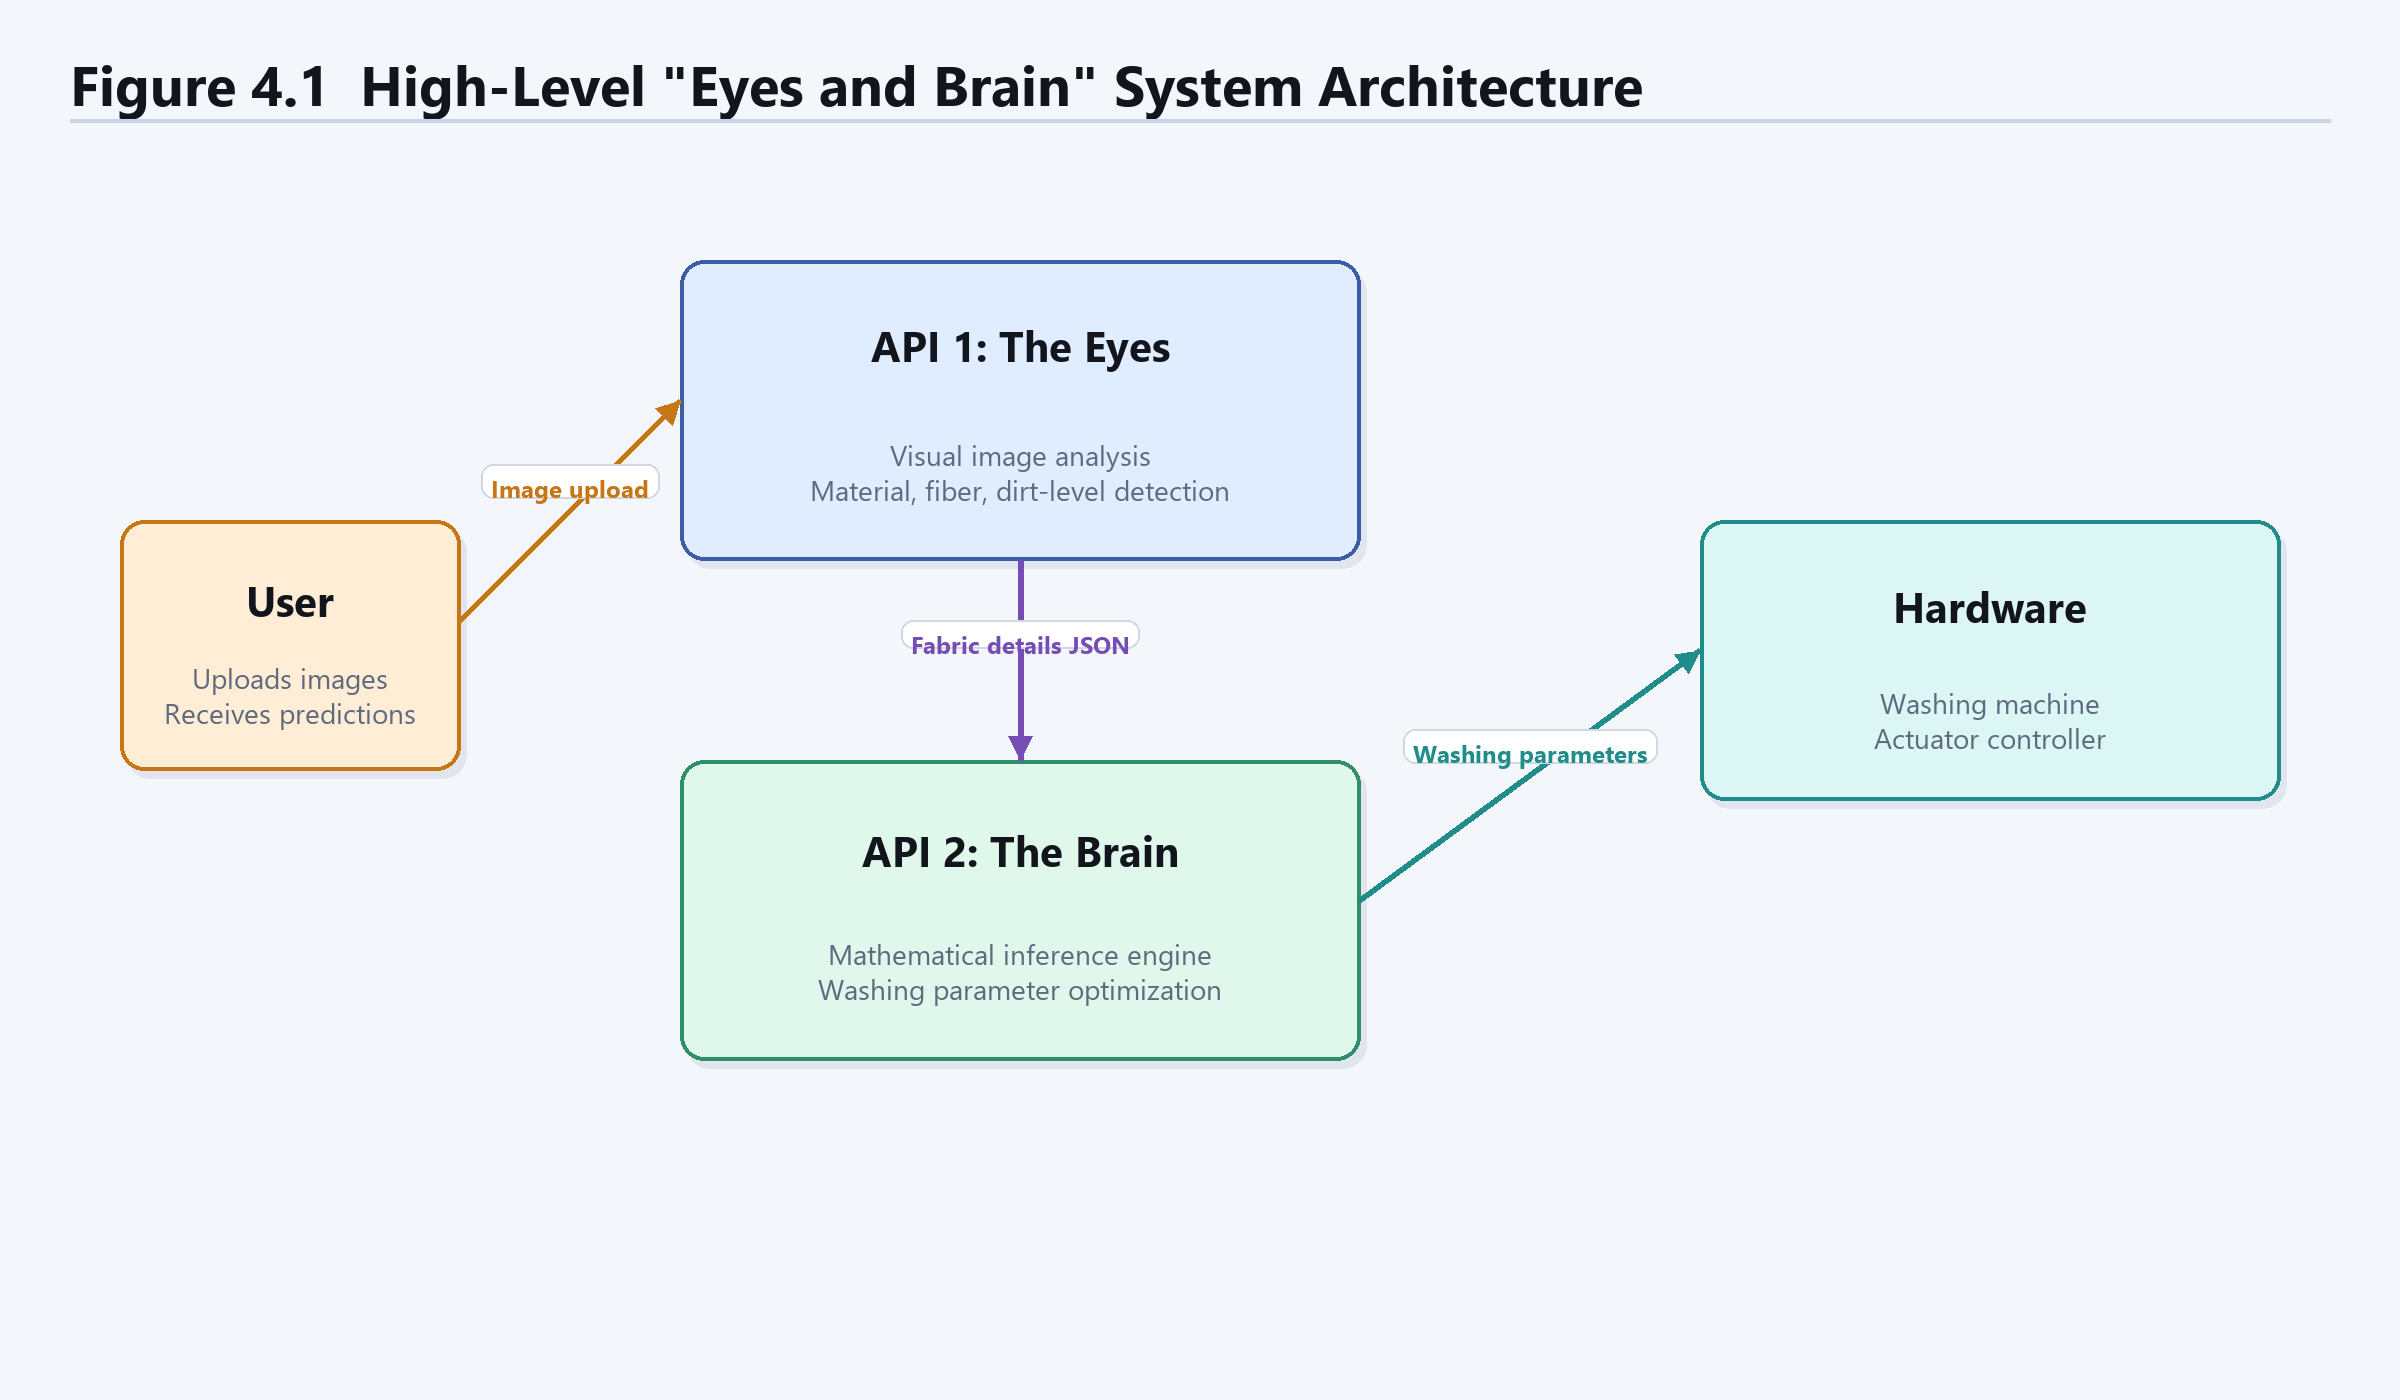
\includegraphics[width=0.9\textwidth]{img/c4diagram1.png}
    \caption{High-Level ``Eyes and Brain'' System Architecture}
    \label{fig:eyes_brain}
\end{figure}
This diagram illustrates the fundamental architectural split of the system. The ``Eyes'' (API 1) handle the visual input through image processing and AI-driven fabric identification, while the ``Brain'' (API 2) performs the logical reasoning and mathematical scaling required to determine safe and effective washing parameters. This separation ensures that the complex task of computer vision does not interfere with the precision required for hardware control.


\section{Data Flow Diagram (DFD)}

\subsection{DFD Level 0 (Context Diagram)}
\begin{figure}[H]
    \centering
    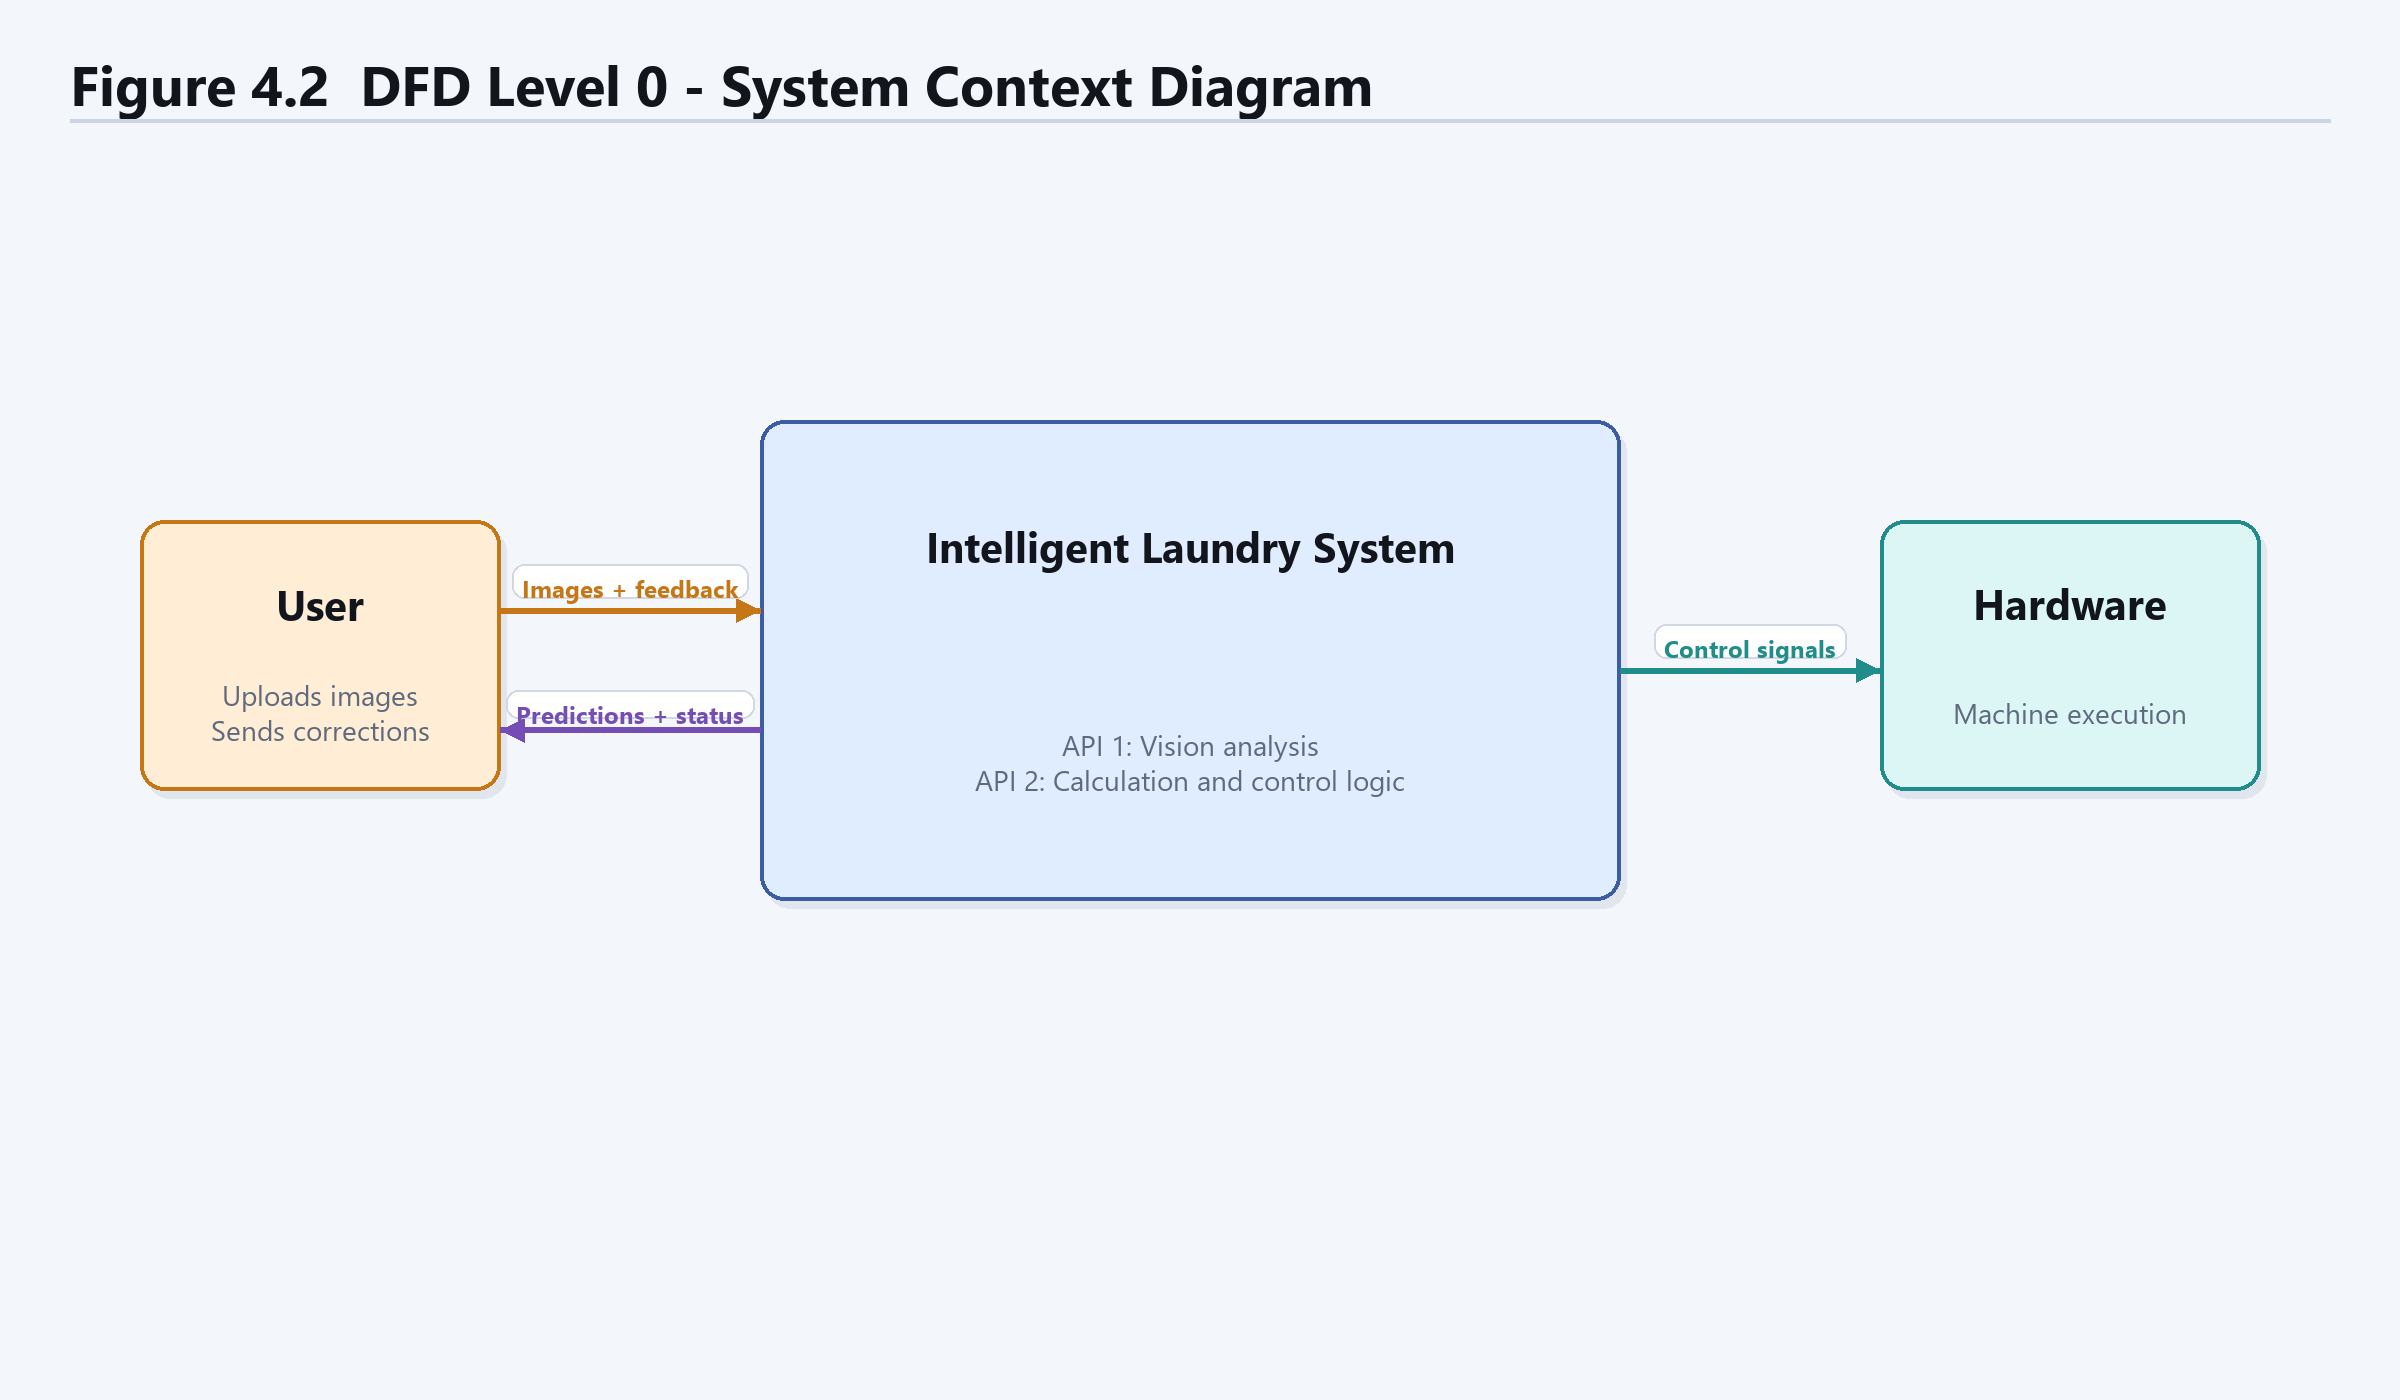
\includegraphics[width=0.8\textwidth]{img/c4diagram2}
    \caption{DFD Level 0 – System Context Diagram}
    \label{fig:dfd0}
\end{figure}
The Context Diagram (Level 0 DFD) defines the boundaries of the Intelligent Laundry System. It shows the system as a single process interacting with three external entities: the User, who provides images and receives status; the AI System (Gemini), which provides fabric analysis; and the Washing Machine Hardware, which receives control signals and reports back the cycle progress.


\subsection{DFD Level 1}
\begin{figure}[H]
    \centering
    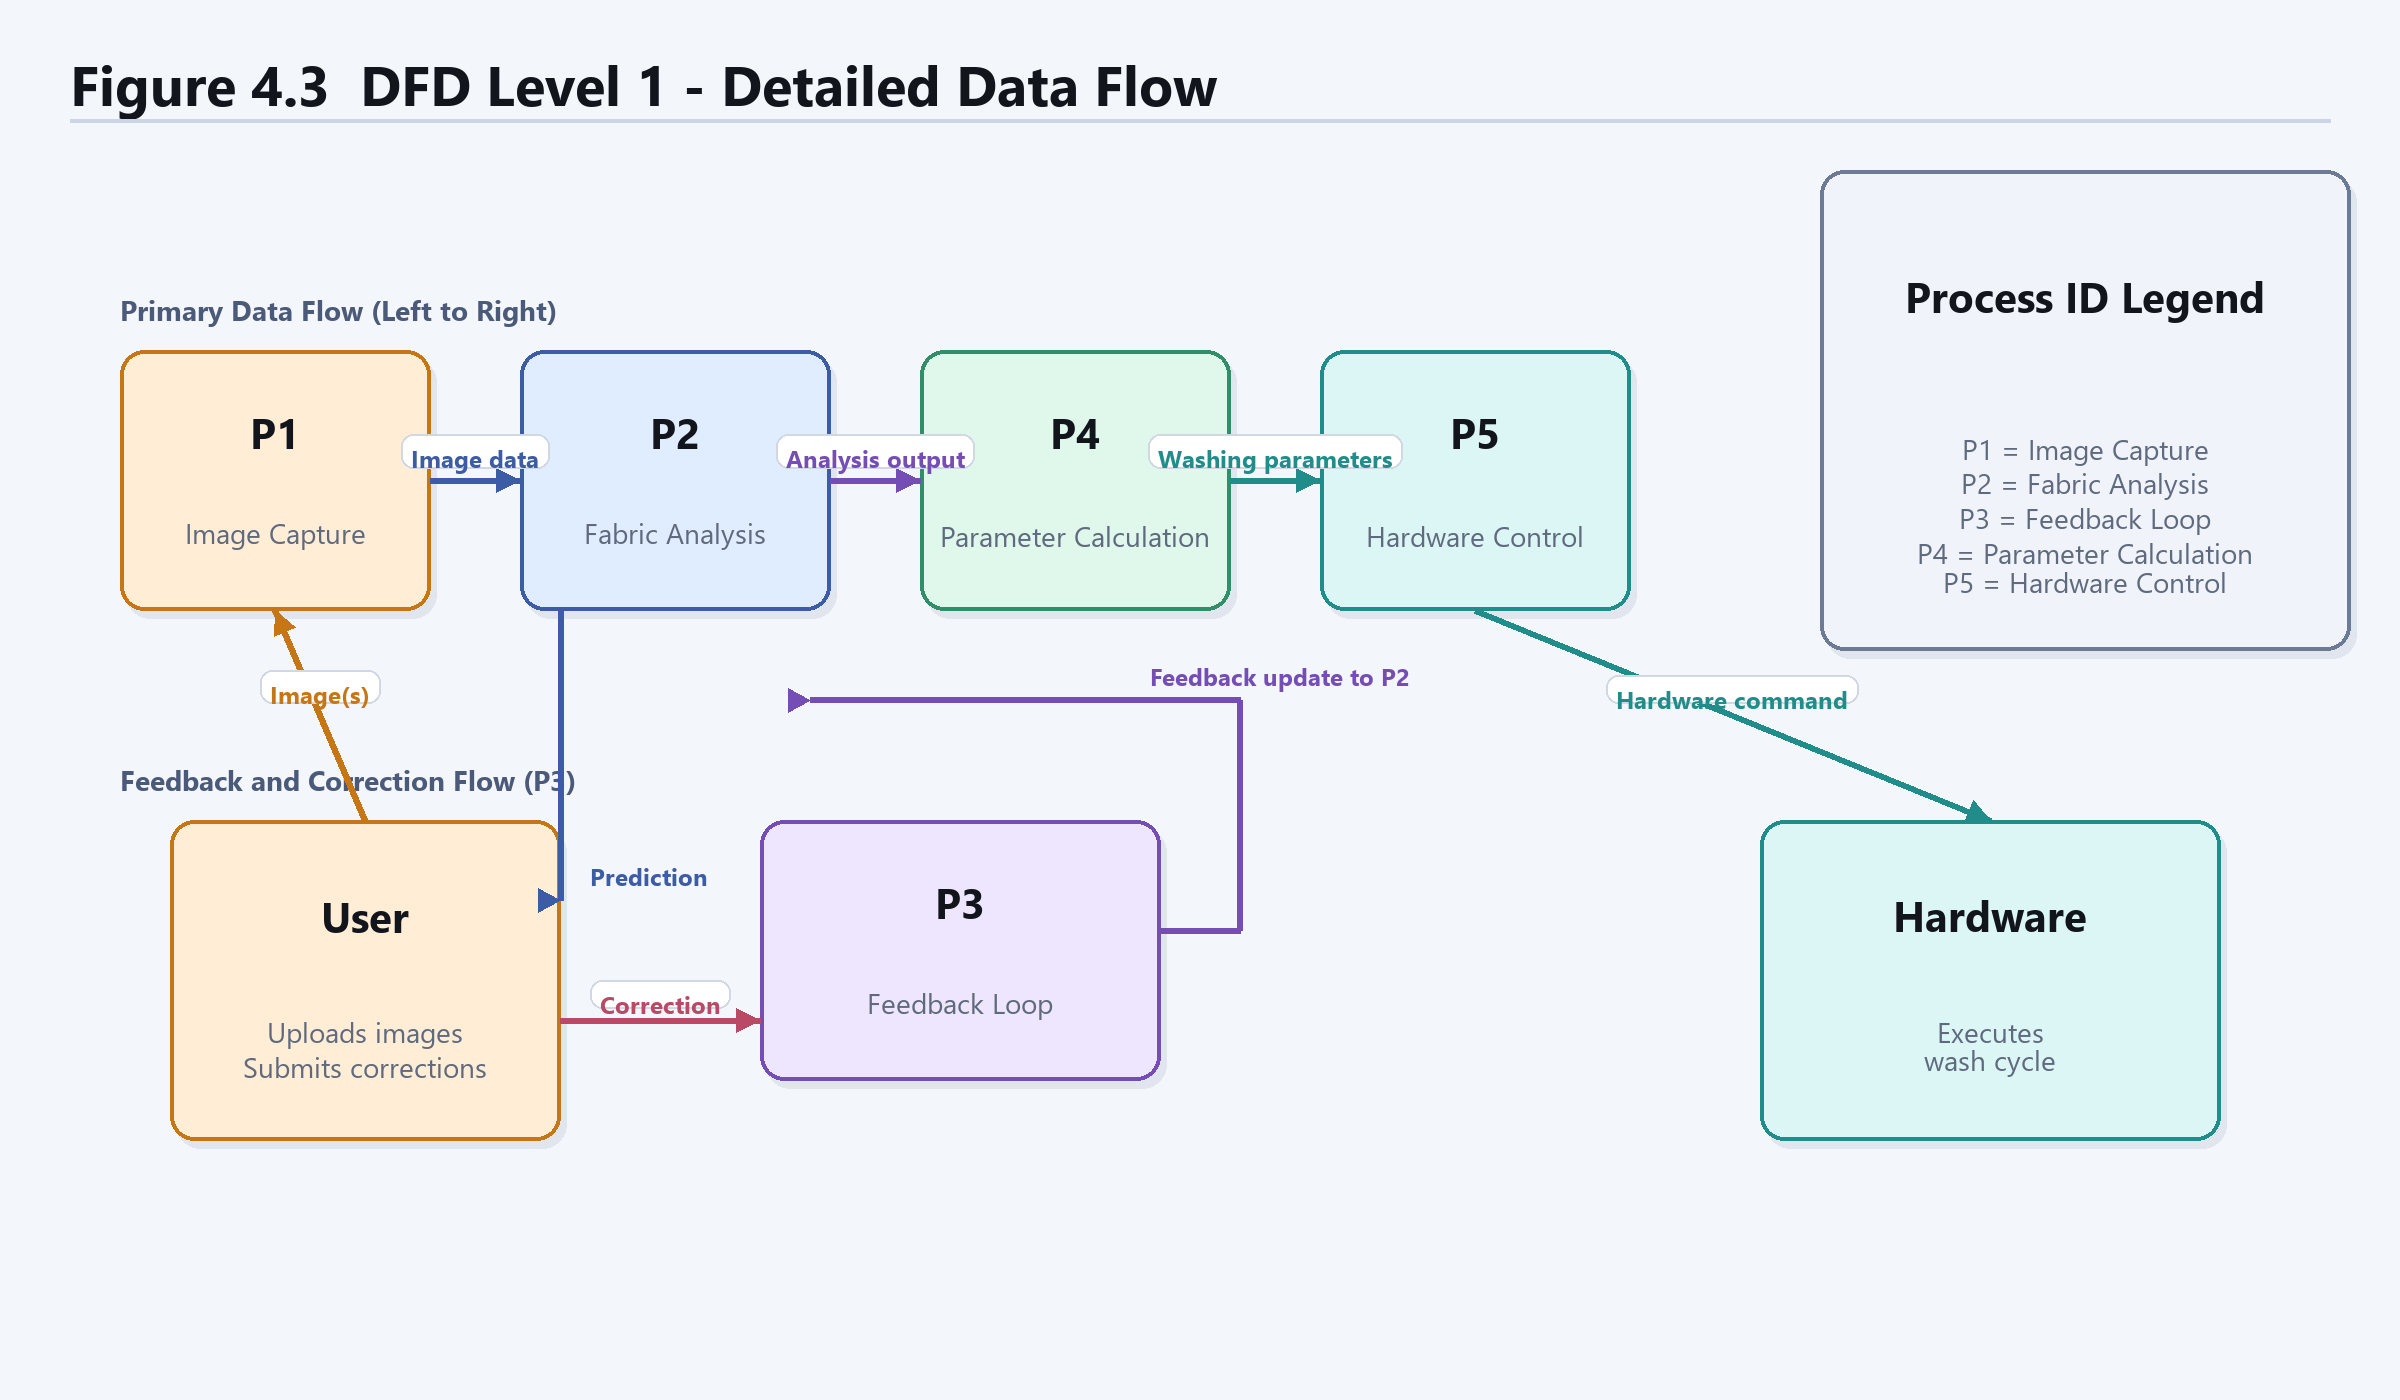
\includegraphics[width=\textwidth]{img/c4diagram3}
    \caption{DFD Level 1 – Detailed Data Flow}
    \label{fig:dfd1}
\end{figure}

The Detailed Data Flow (Level 1 DFD) breaks down the system into five core processes. It begins with \textbf{P1: Image Capture}, where the user’s command triggers the camera feed to capture up to five garment images. These images are passed to \textbf{P2: Fabric Analysis (API 1)}, which utilizes the Gemini vision model to determine the fabric type, fiber category, and dirt level. If a misclassification occurs, \textbf{P3: Feedback Loop} allows the user to submit corrections, providing refined data for a retry. Once the analysis is finalized, \textbf{P4: Parameter Calculation (API 2)} applies the load scaling algorithm to these inputs to derive optimal settings for temperature, water level, detergent, and cycle timings. Finally, in \textbf{P5: Hardware Control}, these combined safe parameters are translated into specific electrical signals to drive the washing machine’s motor and valves.


\section{Use Case Diagram}
\begin{figure}[H]
    \centering
    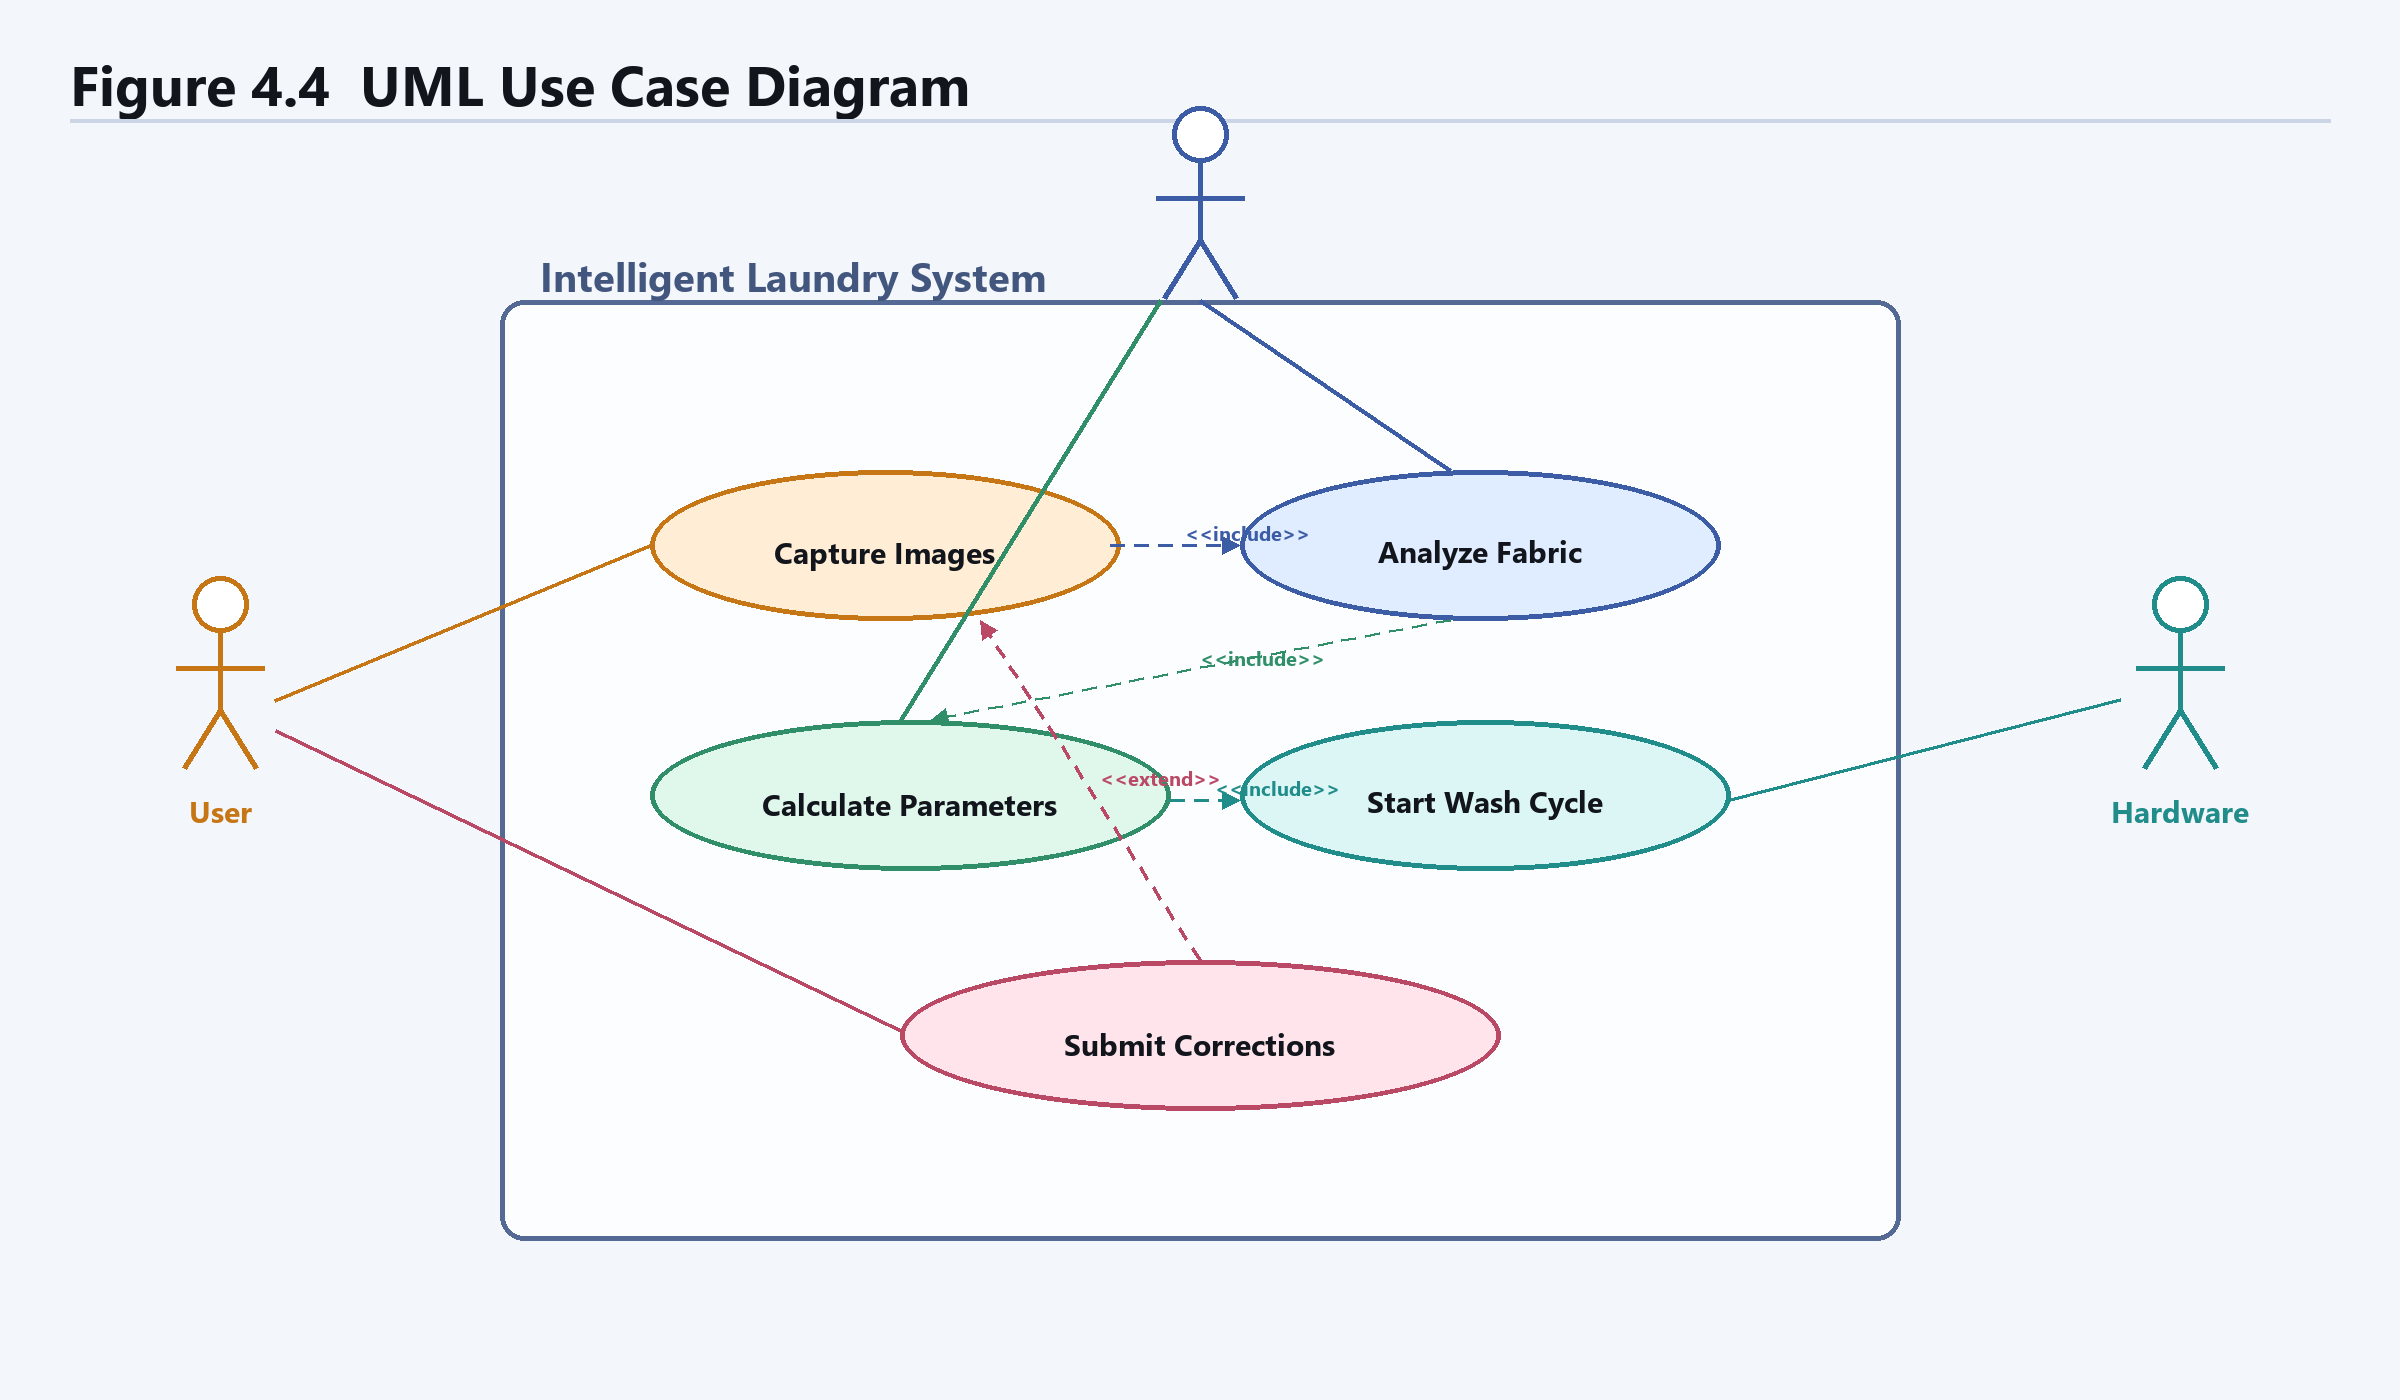
\includegraphics[width=0.9\textwidth]{img/c4diagram4}
    \caption{UML Use Case Diagram}
    \label{fig:usecase}
\end{figure}
The Use Case Diagram identifies the primary interactions between the system's actors and its functional components. The User remains the central actor, initiating garment scans, reviewing AI results, and occasionally providing correction feedback. The AI System (Gemini) acts as a supporting actor for fabric analysis, while the Washing Machine Hardware executes the resulting use cases such as starting the wash cycle and reporting real-time progress.


\textbf{Actors:}
\begin{itemize}
    \item User
    \item AI System (Gemini)
    \item Washing Machine Hardware
\end{itemize}

\textbf{Use Cases:}
\begin{itemize}
    \item Capture up to 5 garment images
    \item Analyze fabric types
    \item Submit correction feedback
    \item Calculate washing parameters for mixed loads
    \item Start washing cycle
    \item Monitor progress
\end{itemize}

\section{API Design}

\subsection{API 1: Clothing Material Identifier}
\textbf{Endpoint:} \texttt{/predict/}\\
\textbf{Method:} POST\\
\textbf{Input:} Up to 5 images (multipart/form-data)\\
\textbf{Output:} JSON array with fabric analysis for each image

% No image for JSON structure – shown as listing
\begin{lstlisting}[caption=API 1 Response Format, label=lst:api1, language=JSON]
{
  "total_images": 2,
  "results": [
    {
      "filename": "shirt.jpg",
      "material_type": "Cotton Denim",
      "fiber_category": "Natural",
      "description": "Highly durable diagonal twill. Excellent breathability, low wrinkle resistance.",
      "dirt_level": 4,
      "confidence_score": 0.94
    },
    {
      "filename": "scarf.jpg",
      "material_type": "Silk",
      "fiber_category": "Natural",
      "description": "Luxurious smooth fiber with high luster. Delicate, requires gentle handling.",
      "dirt_level": 2,
      "confidence_score": 0.89
    }
  ]
}
\end{lstlisting}

\subsection{API 2: Washing Parameter Predictor}
\textbf{Endpoint:} \texttt{/predict/}\\
\textbf{Method:} POST\\
\textbf{Input:} API 1 output JSON\\
\textbf{Output:} Combined washing parameters for the entire load

\begin{lstlisting}[caption=API 2 Response Format, label=lst:api2, language=JSON]
{
  "temperature_setting": 30,
  "water_level": 35,
  "detergent_amount": 35,
  "soak_time": 10,
  "spin_time": 8,
  "mechanical_action": "Gentle"
}
\end{lstlisting}

\section{Load Scaling Algorithm for Mixed Fabrics}
The most significant engineering challenge was safely processing mixed loads containing different fabric types. The system implements a \textbf{Concentration-Based Load Scaling Algorithm} with strict safety priorities.

\subsection{Algorithm Rules}
\begin{figure}[H]
    \centering
    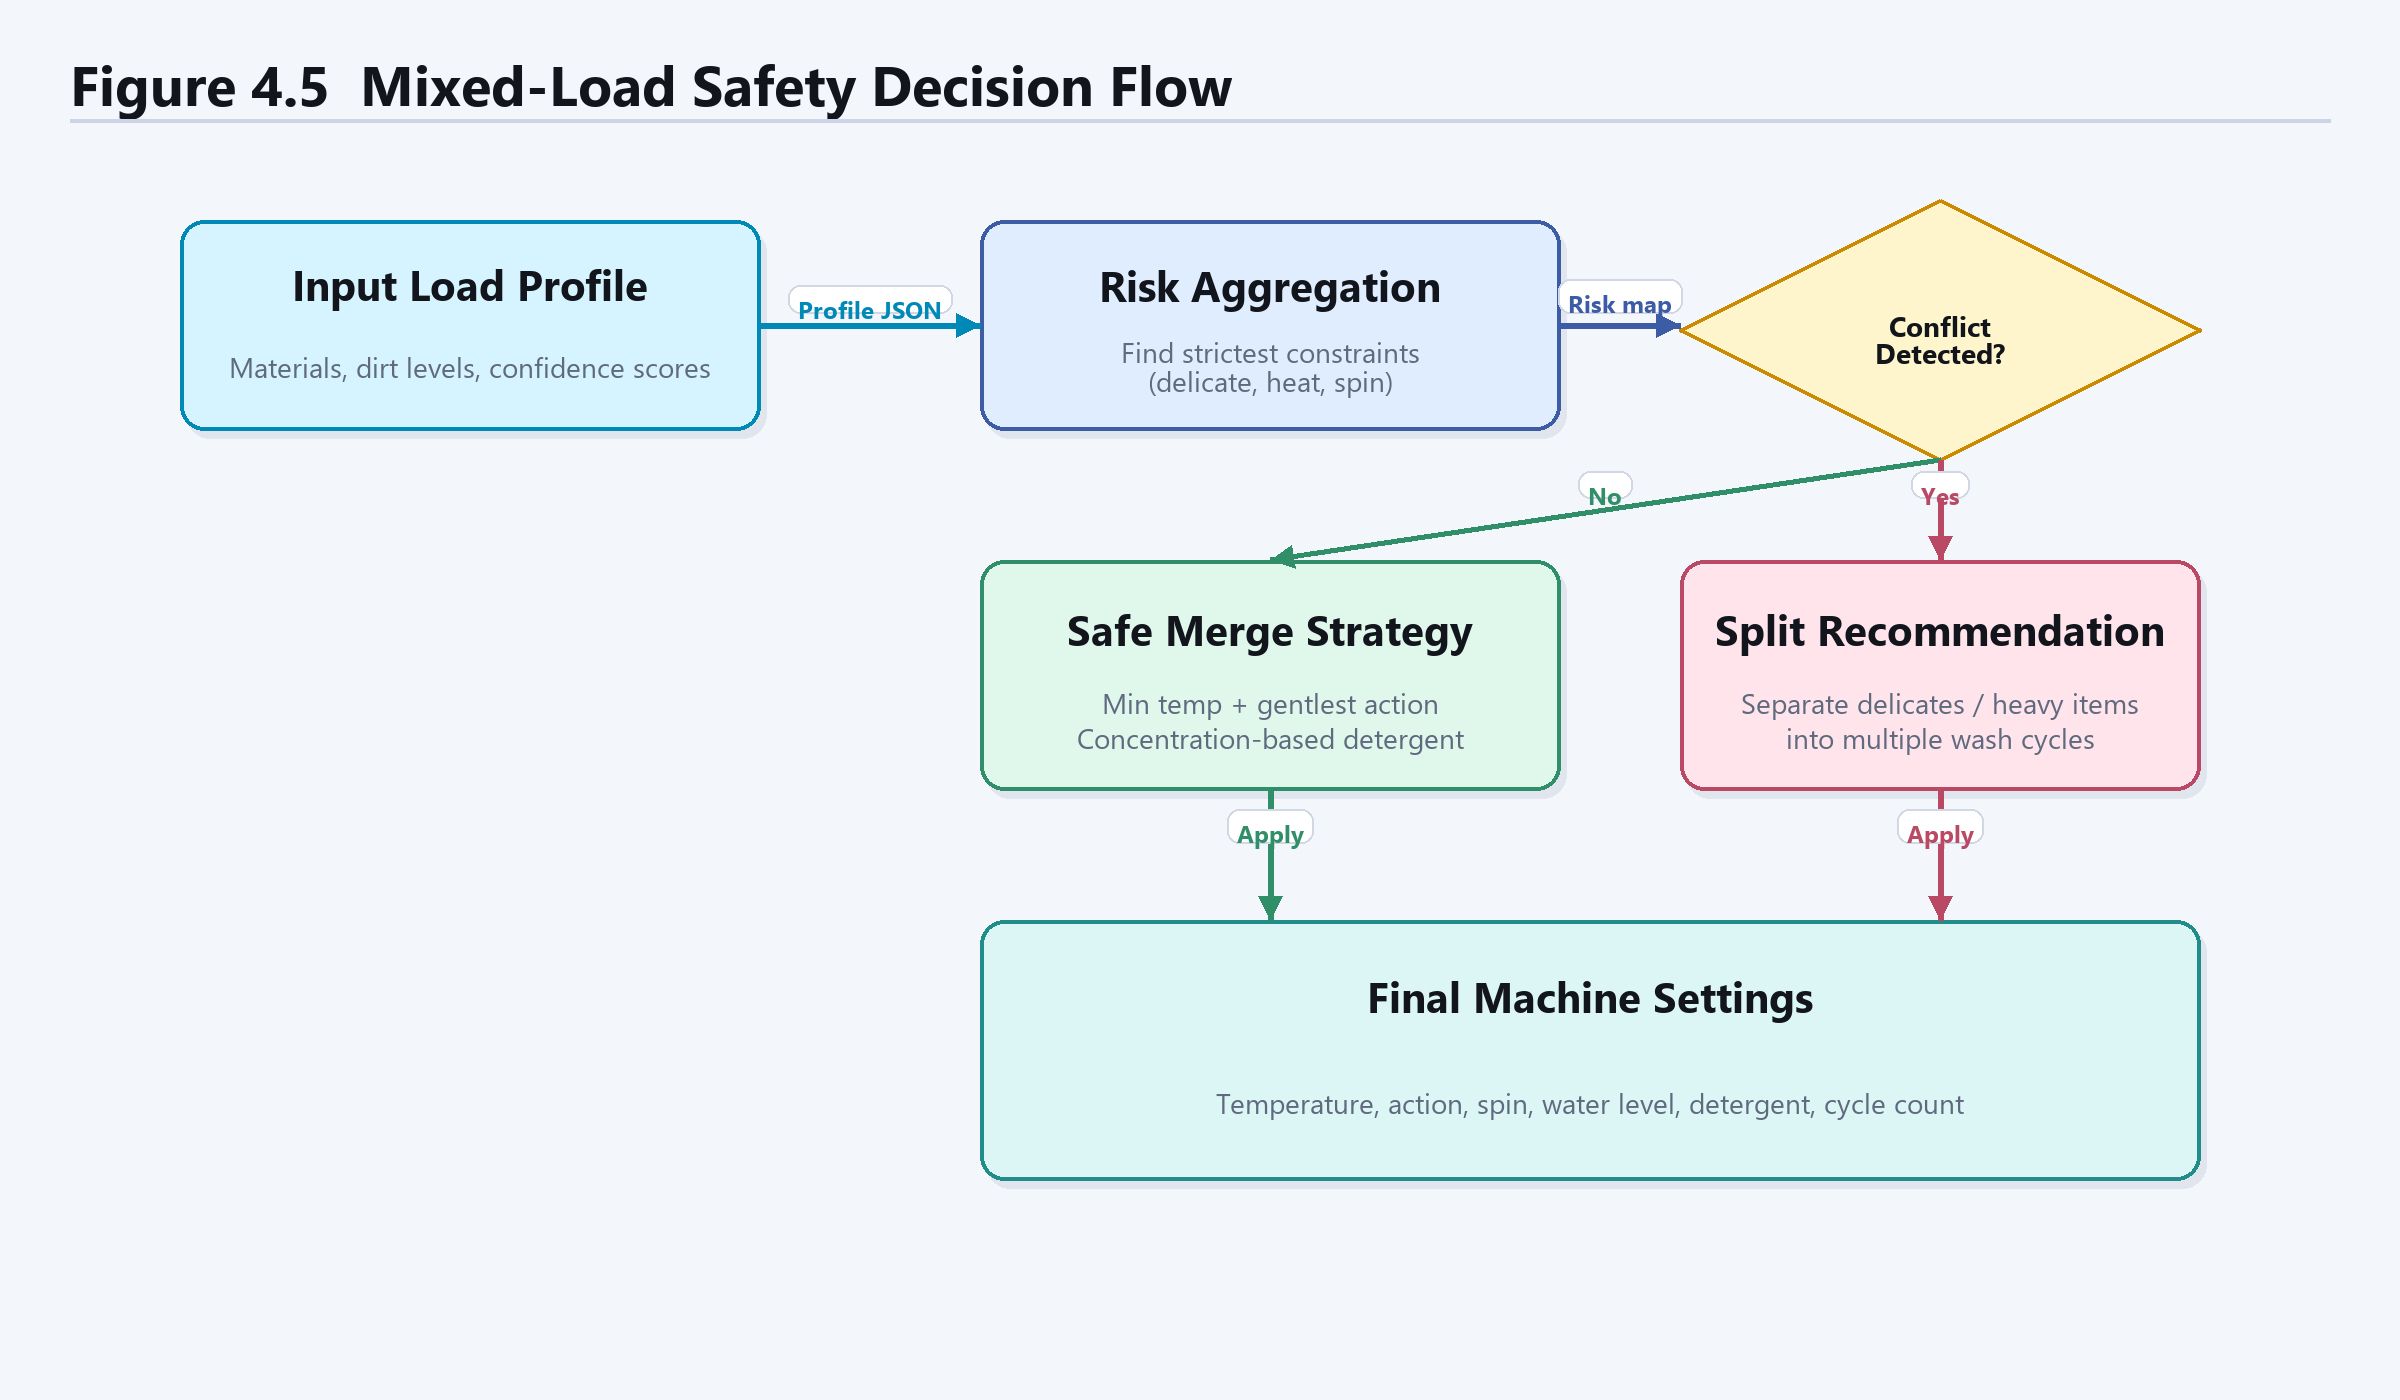
\includegraphics[width=0.8\textwidth]{img/c4diagram7}
    \caption{Mixed Load Safety Decision Flow}
    \label{fig:loadscaling}
\end{figure}
This decision flow diagram details the logic used when the system encounters multiple items in a single load. The core philosophy is ``safety first,'' where the system evaluates the requirements of every item and automatically selects the most conservative settings—such as the lowest temperature and gentlest mechanical action—to ensure that no delicate garment is damaged during a mixed-fabric wash cycle.


To manage mixed loads effectively, the system follows a set of strict parameter selection rules designed for fabric safety and cleaning efficiency. For temperature and spin time, the algorithm always selects the minimum value among all garments in the load to prevent heat-induced shrinking or mechanical stretching of delicate fibers. The water level is dynamically calculated based on the total load size but is strictly capped at a 60-liter maximum to prevent overflow. Mechanical action is determined by the most sensitive item, ensuring the gentlest required agitation is used for the entire batch. Conversely, detergent volume is calculated based on the heaviest soil level identified in the load, ensuring thorough cleaning without wasting chemicals.




The system is engineered to handle various edge cases gracefully through predefined handling strategies. If a non-clothing image is accidentally uploaded, the visual analysis layer (API 1) identifies the error and prevents the subsequent parameter calculation from being triggered. In scenarios involving highly diverse loads with five different fabric types, the algorithm defaults to the safest possible parameters for the most delicate item identified. For garments with extremely high soil levels (level 5), the system proactively increases detergent volume and soak durations while strictly maintaining the fabric-safe temperature limits. Finally, if the total load size exceeds normal capacity, the system applies a hard cap of 60 liters on the water level to ensure safe operation.


\section{Feedback Loop Design}
The system incorporates a Human-in-the-Loop (HITL) feedback mechanism for continuous improvement.

\begin{figure}[H]
    \centering
    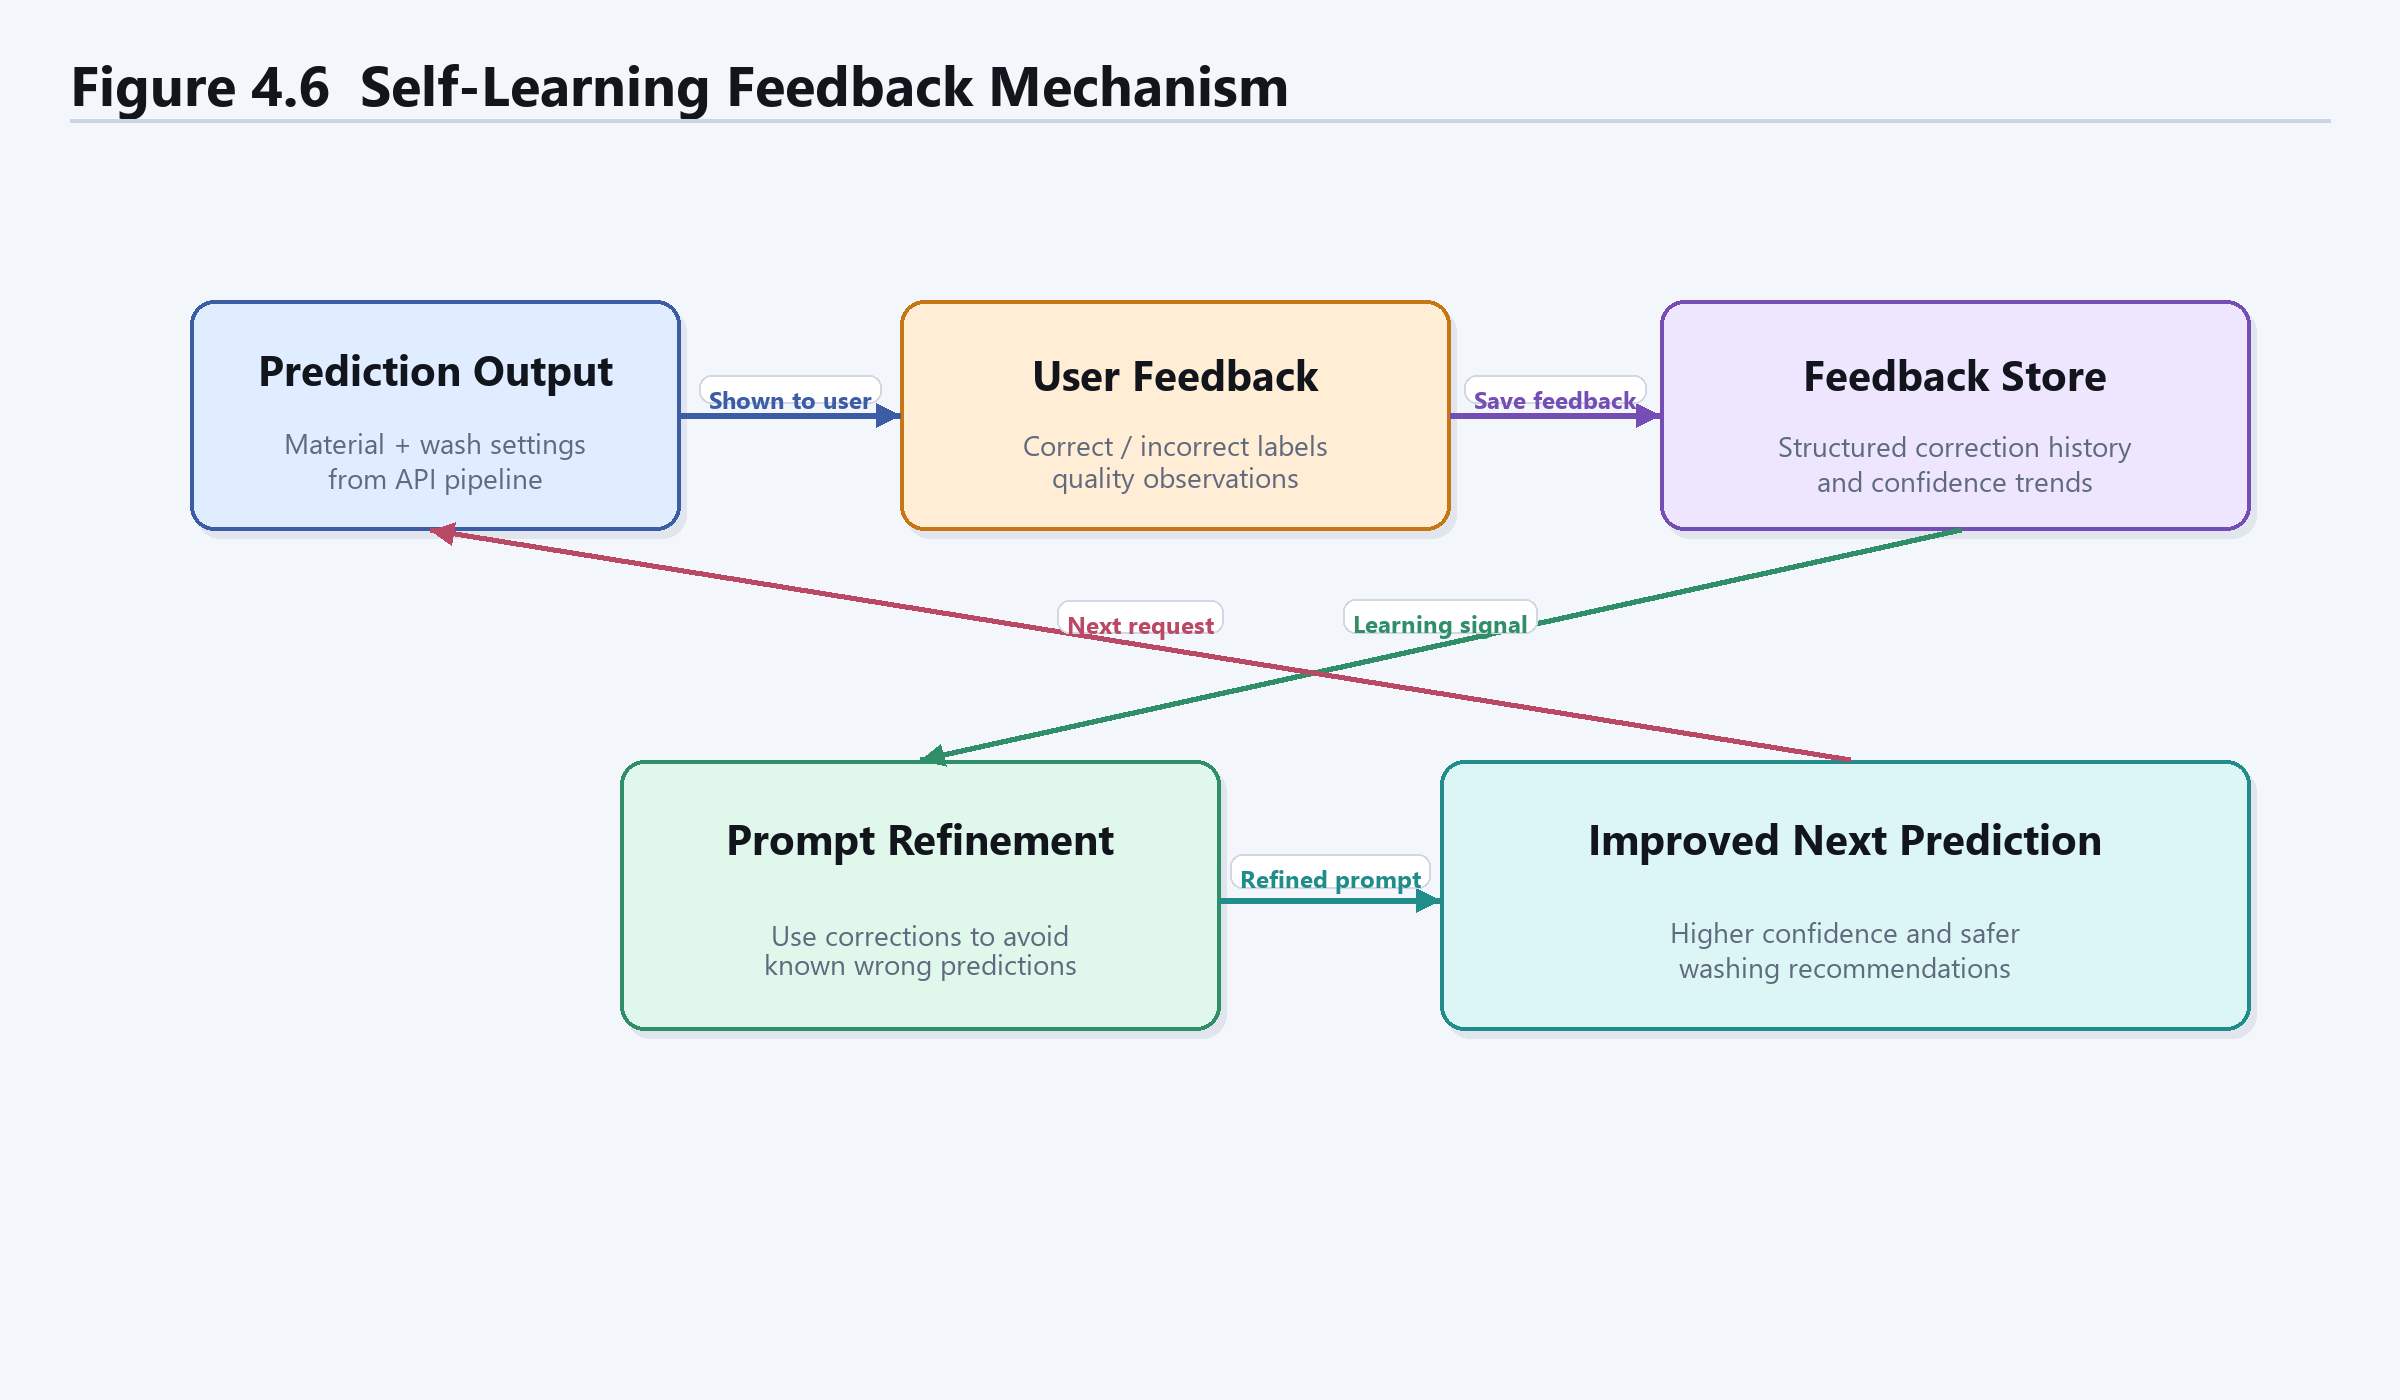
\includegraphics[width=0.9\textwidth]{img/c4diagram8}
    \caption{Self-Learning Feedback Mechanism}
    \label{fig:feedback}
\end{figure}

\textbf{Process:}
\begin{enumerate}
    \item AI makes prediction with confidence score
    \item User reviews result
    \item If incorrect, user submits correction to \texttt{/feedback} endpoint
    \item Correction stored in database
    \item On retry, system prompts AI with: ``IMPORTANT: 'Cotton' was INCORRECT! Look more carefully...''
    \item AI self-corrects and provides improved accuracy
\end{enumerate}

\section{Rate Limiting and Failover Design}
To ensure system reliability and prevent crashes from request bursts:

\begin{figure}[H]
    \centering
    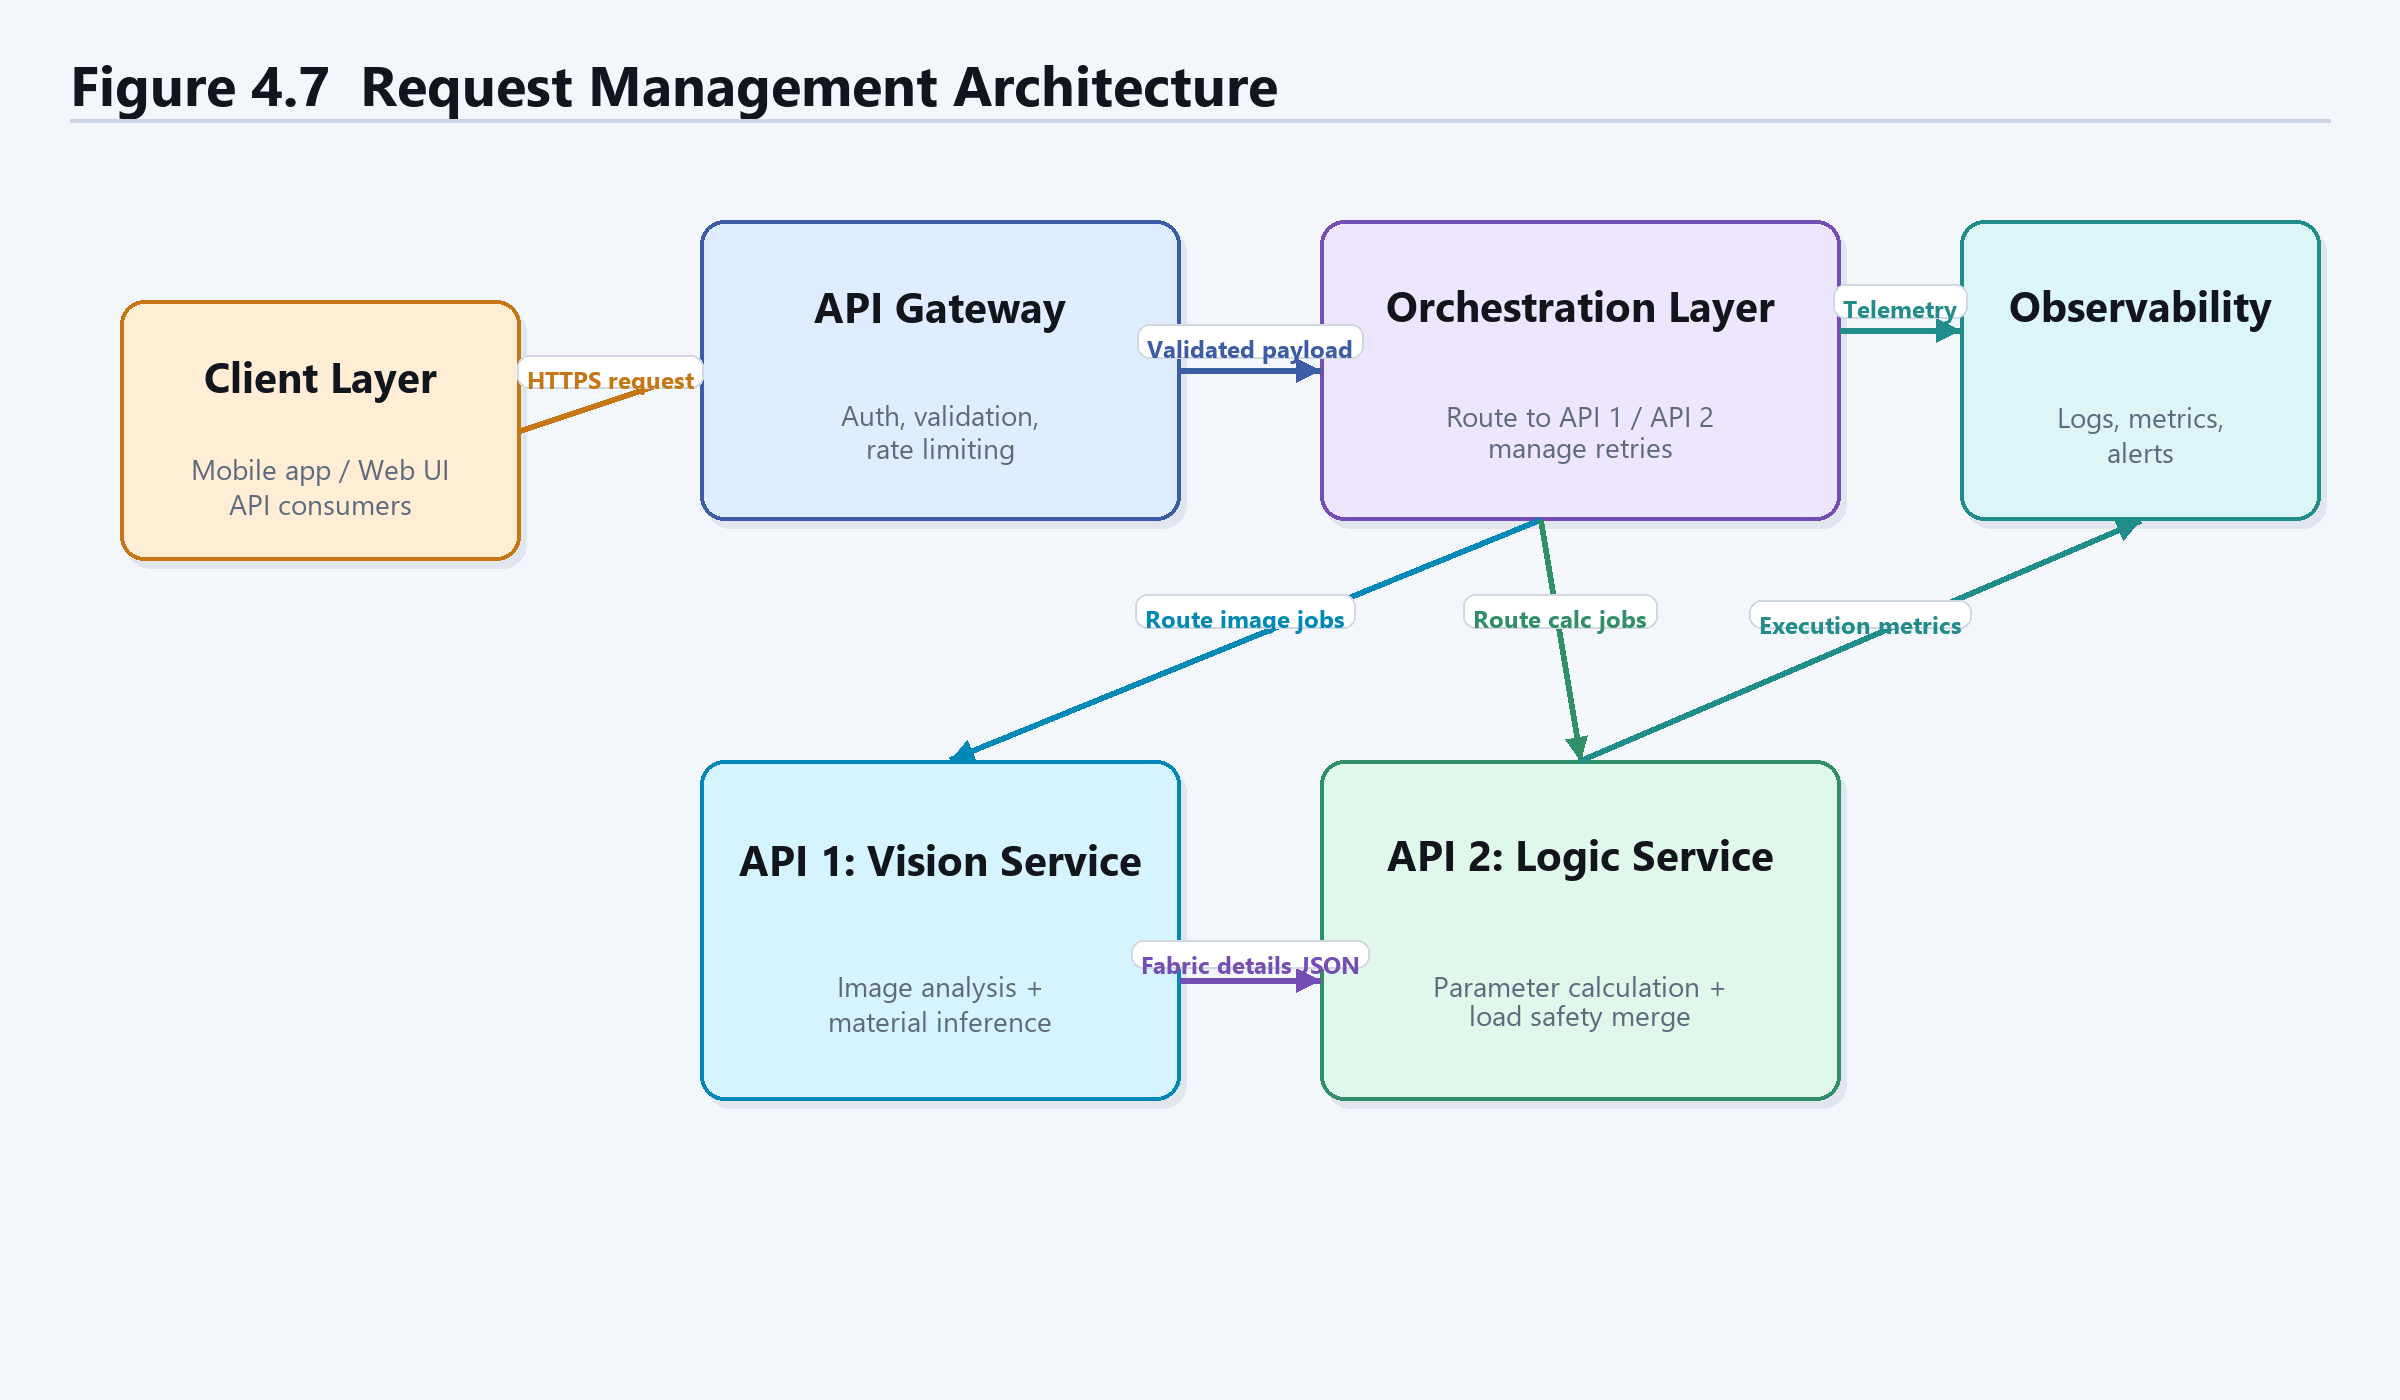
\includegraphics[width=0.9\textwidth]{img/c4diagram9}
    \caption{Request Management Architecture}
    \label{fig:ratelimit}
\end{figure}

\textbf{Implementation Features:}
\begin{itemize}
    \item \textbf{Rate Limiting:} Maximum requests per minute per user
    \item \textbf{Automatic Failover:} If primary \texttt{gemini-1.5-flash} model is overwhelmed, system gracefully waits or switches to backup model
    \item \textbf{Queue Management:} Requests are queued during high traffic
    \item \textbf{Timeout Handling:} Failed requests are retried with exponential backoff
\end{itemize}

\section{End-to-End Validation Design}
To prove system integration, an automated test pipeline validates both APIs working in harmony.

\begin{figure}[H]
    \centering
    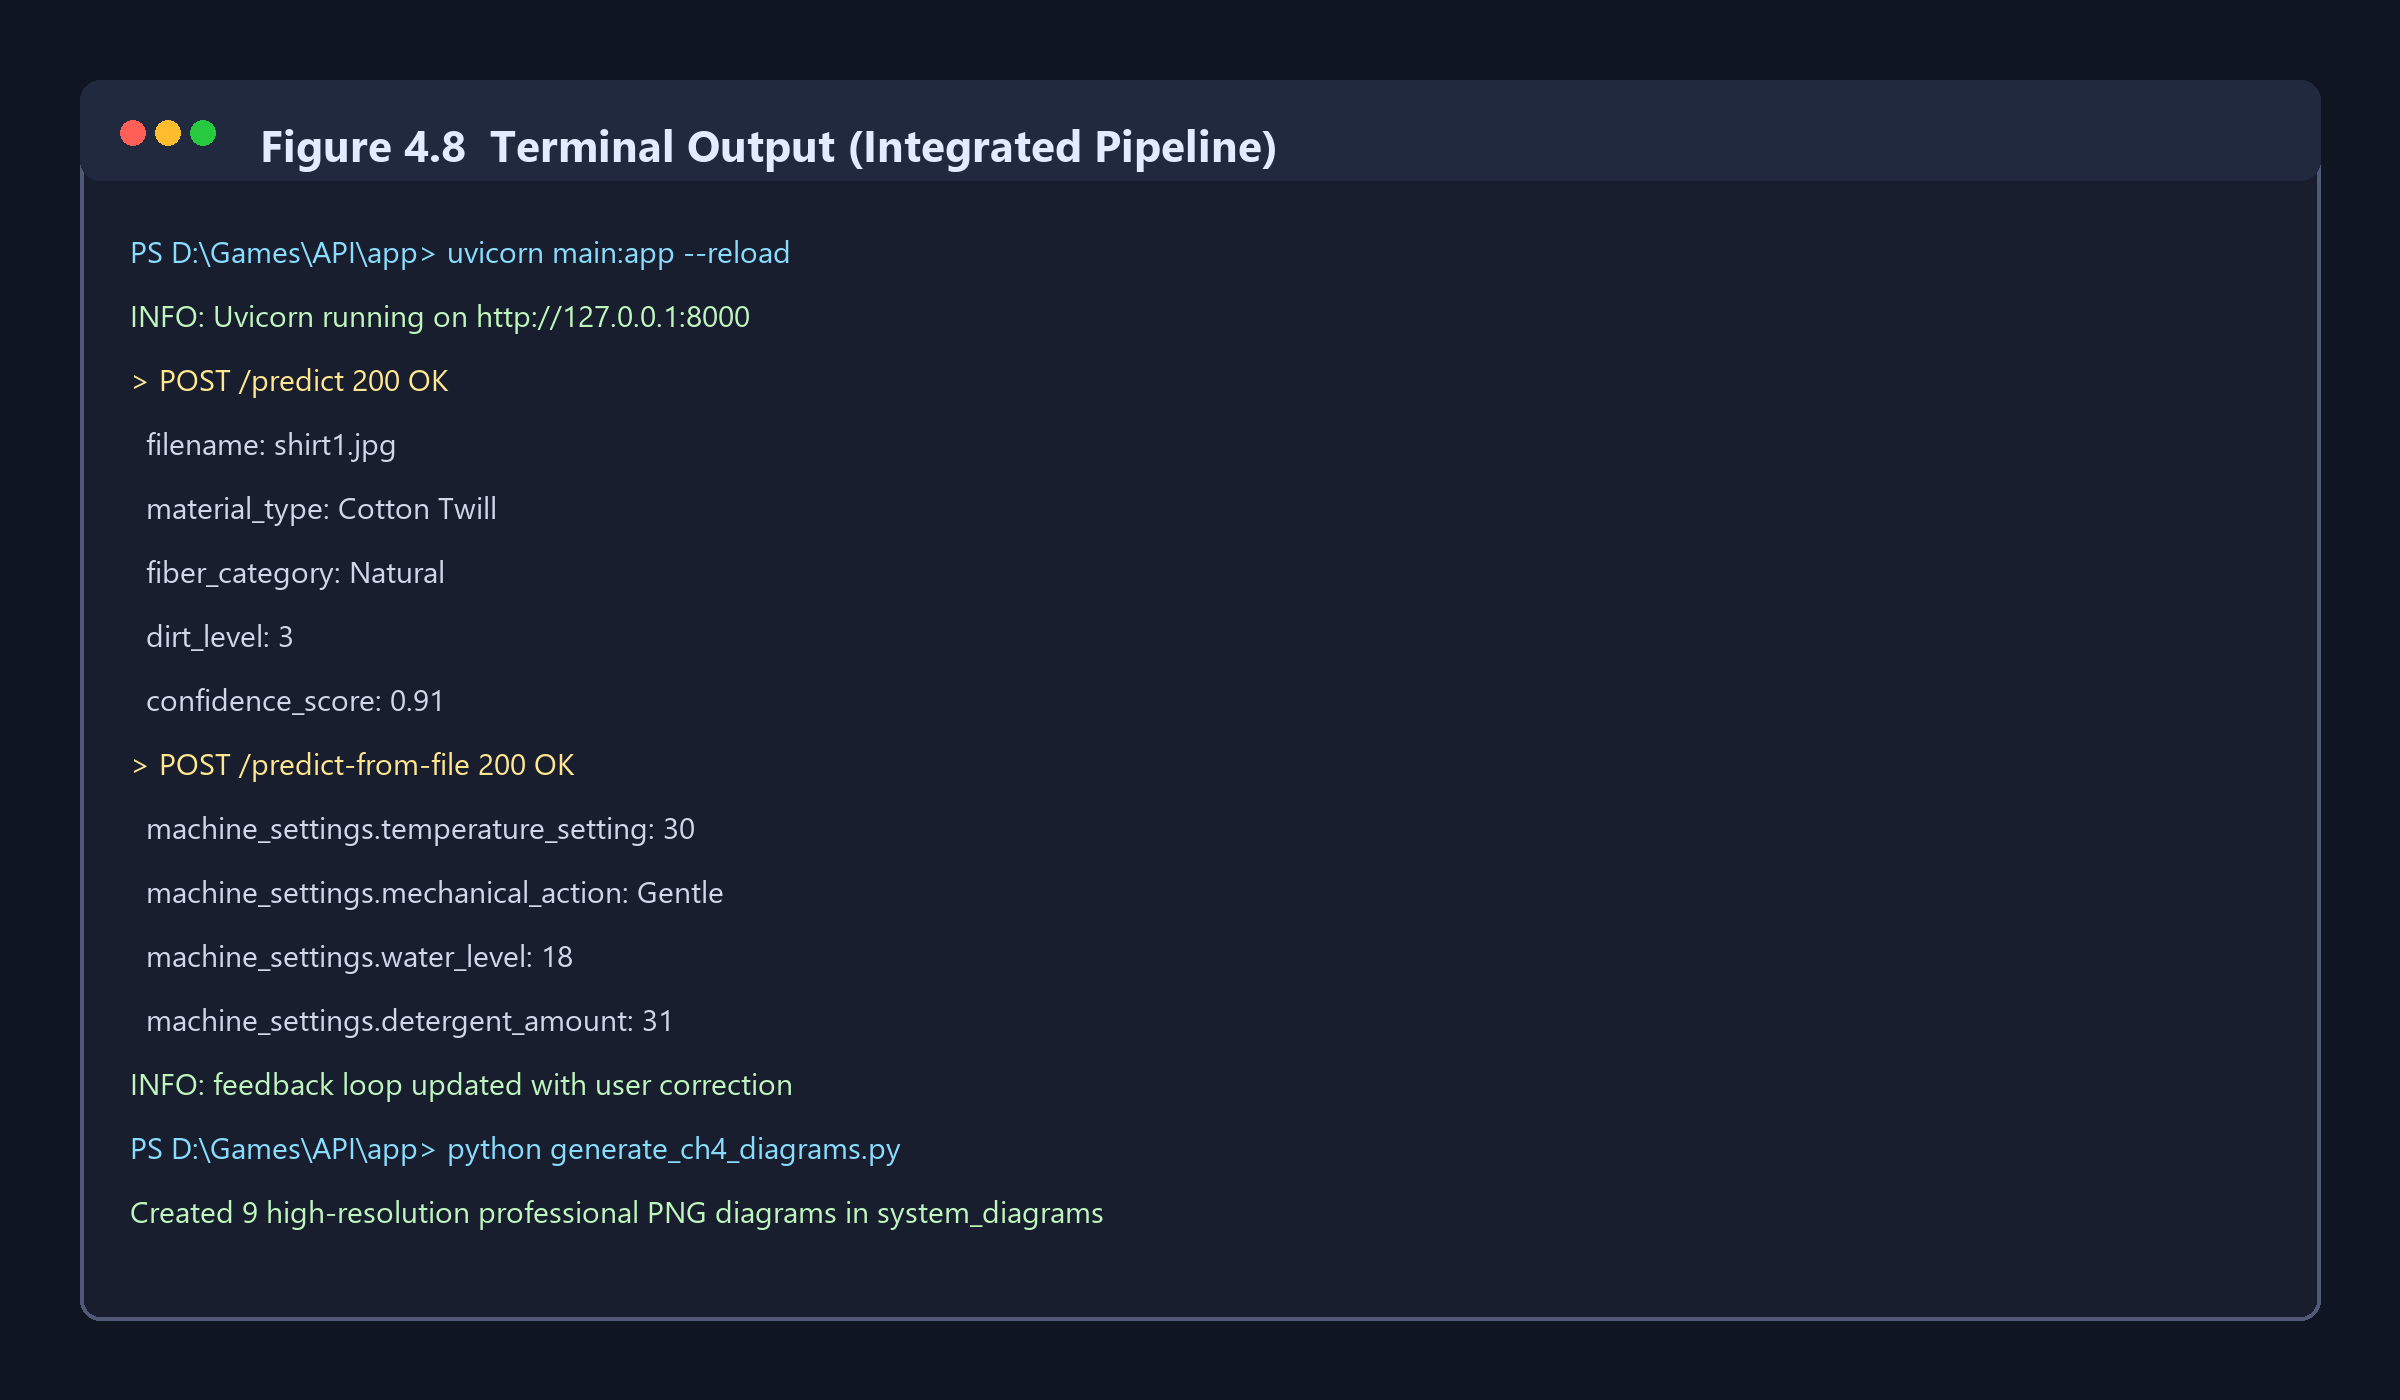
\includegraphics[width=0.9\textwidth]{img/c4diagram10}
    \caption{Terminal Output – Successful End-to-End Test}
    \label{fig:testoutput}
\end{figure}



\section{Hardware Control Interface Design}
The hardware interface translates API 2 parameters into Arduino control signals.

\begin{figure}[H]
    \centering
    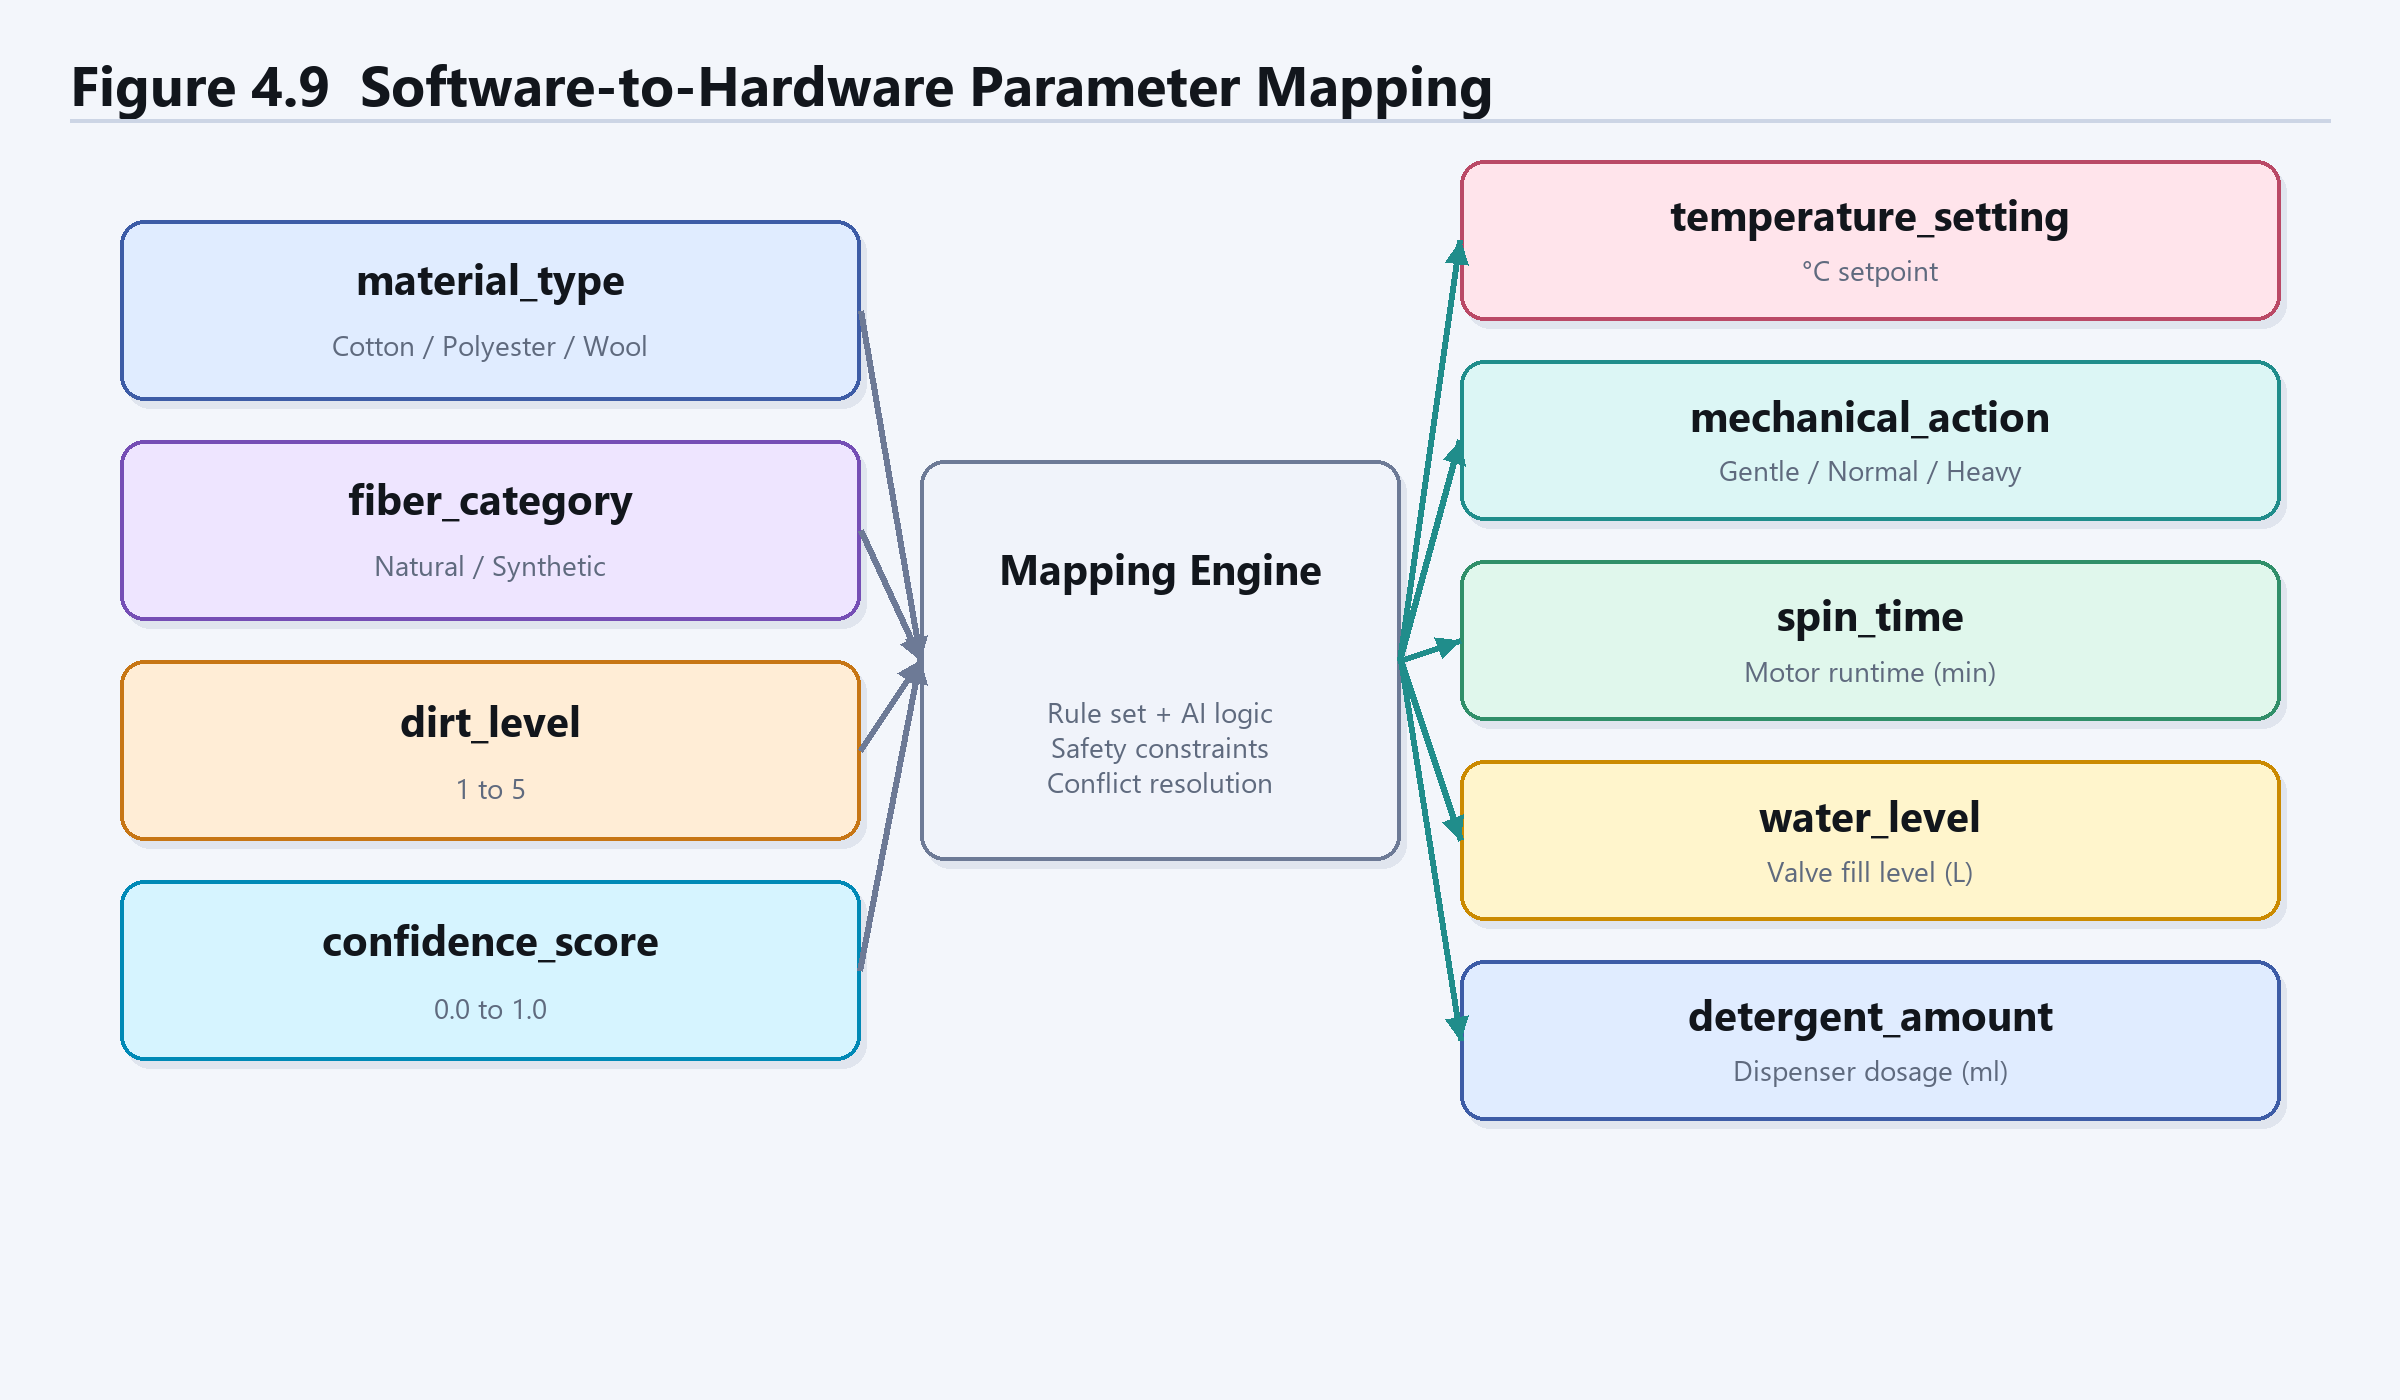
\includegraphics[width=\textwidth]{img/c4diagram11}
    \caption{Software-to-Hardware Parameter Mapping}
    \label{fig:hardware_map}
\end{figure}

The Software-to-Hardware Parameter Mapping illustrates how the logical wash settings are converted into physical machine actions. The temperature setting is mapped to heater control using relays or PWM signals. The water level is achieved by controlling the duration of the water inlet solenoid valve. For detergent dispensing, the system calculates the exact pump activation time using a linear regression model based on the required volume. Soak times are implemented via software timers that keep the motor off for the specified period, while spin times and mechanical actions are executed through precise relay sequences and timing variations that control the motor’s rotation pattern and effective speed.
